\subsection{SOLUCIÓN PLANTEADA}

Para solucionar la problemática planteada, se propone el desarrollo de una
herramienta computacional capaz de tomar datos de forma continua y enviarlos  a
un servidor el cual permita  almacenar, estudiar y muestrear la información en
distintos niveles de profundidad.

Dadas las dificultades de medición expuestas y la carencia de datos continuos
para el análisis exhaustivo, la solución propuesta es una herramienta digital,
diagramada en la Figura \ref{diagrama}, la cual sirve como base, simulación y
prototipo ante  una posible automatización, que al ser modular permite la
utilización del software-herramienta, en combinación con otros proyectos (como
lo puede ser el usar hardware libre Memsio de \textcite{Koene} como fuente de
datos al servidor), con muy pocas modificaciones.

Para esto, se dispone de una base de datos (BBDD externa), proporcionada por un
tercero (empresa dedicada al estudio de la vibración), la cual dará pie a un
análisis estadístico para la obtención de un modelo del compartimento de un
motor eléctrico con distintos niveles de daño y la salida correspondiente dada
por un acelerómetro digital. De esta forma se alimenta el servidor con datos
proporcionados por el modelo y un valor semilla (características del motor,
grado de daño, etc) los cuales se almacenarán en una nueva base de datos (BBDD)
para, posteriormente, ser procesada y  generar 3 niveles de análisis:

%un modelo de la salida de un acelerómetro digital dado el compartimento de un motor eléctrico con distintos niveles de daño.

\begin{itemize}

\item La vista principal, permitirá observar una cantidad específica de
motores, simbolizando los existentes en una planta o piso, y su estado general.

\item La vista específica, dará la información actual e histórica referente a
un único motor previamente seleccionado.

\item La vista exhaustiva se refiere a un análisis en frecuencia de la
vibración de un motor especificado con anterioridad, con la finalidad de
permitir al operador o ingeniero encargado determinar las posibles
averías y sus causas.

\end{itemize}

Y finalmente, toda esta información y opciones se mostrarían a través de una
página Web para facilitar su acceso.

\begin{figure}[htb]
\centering
\caption{Diagrama de la herramienta computacional.}
\label{diagrama}
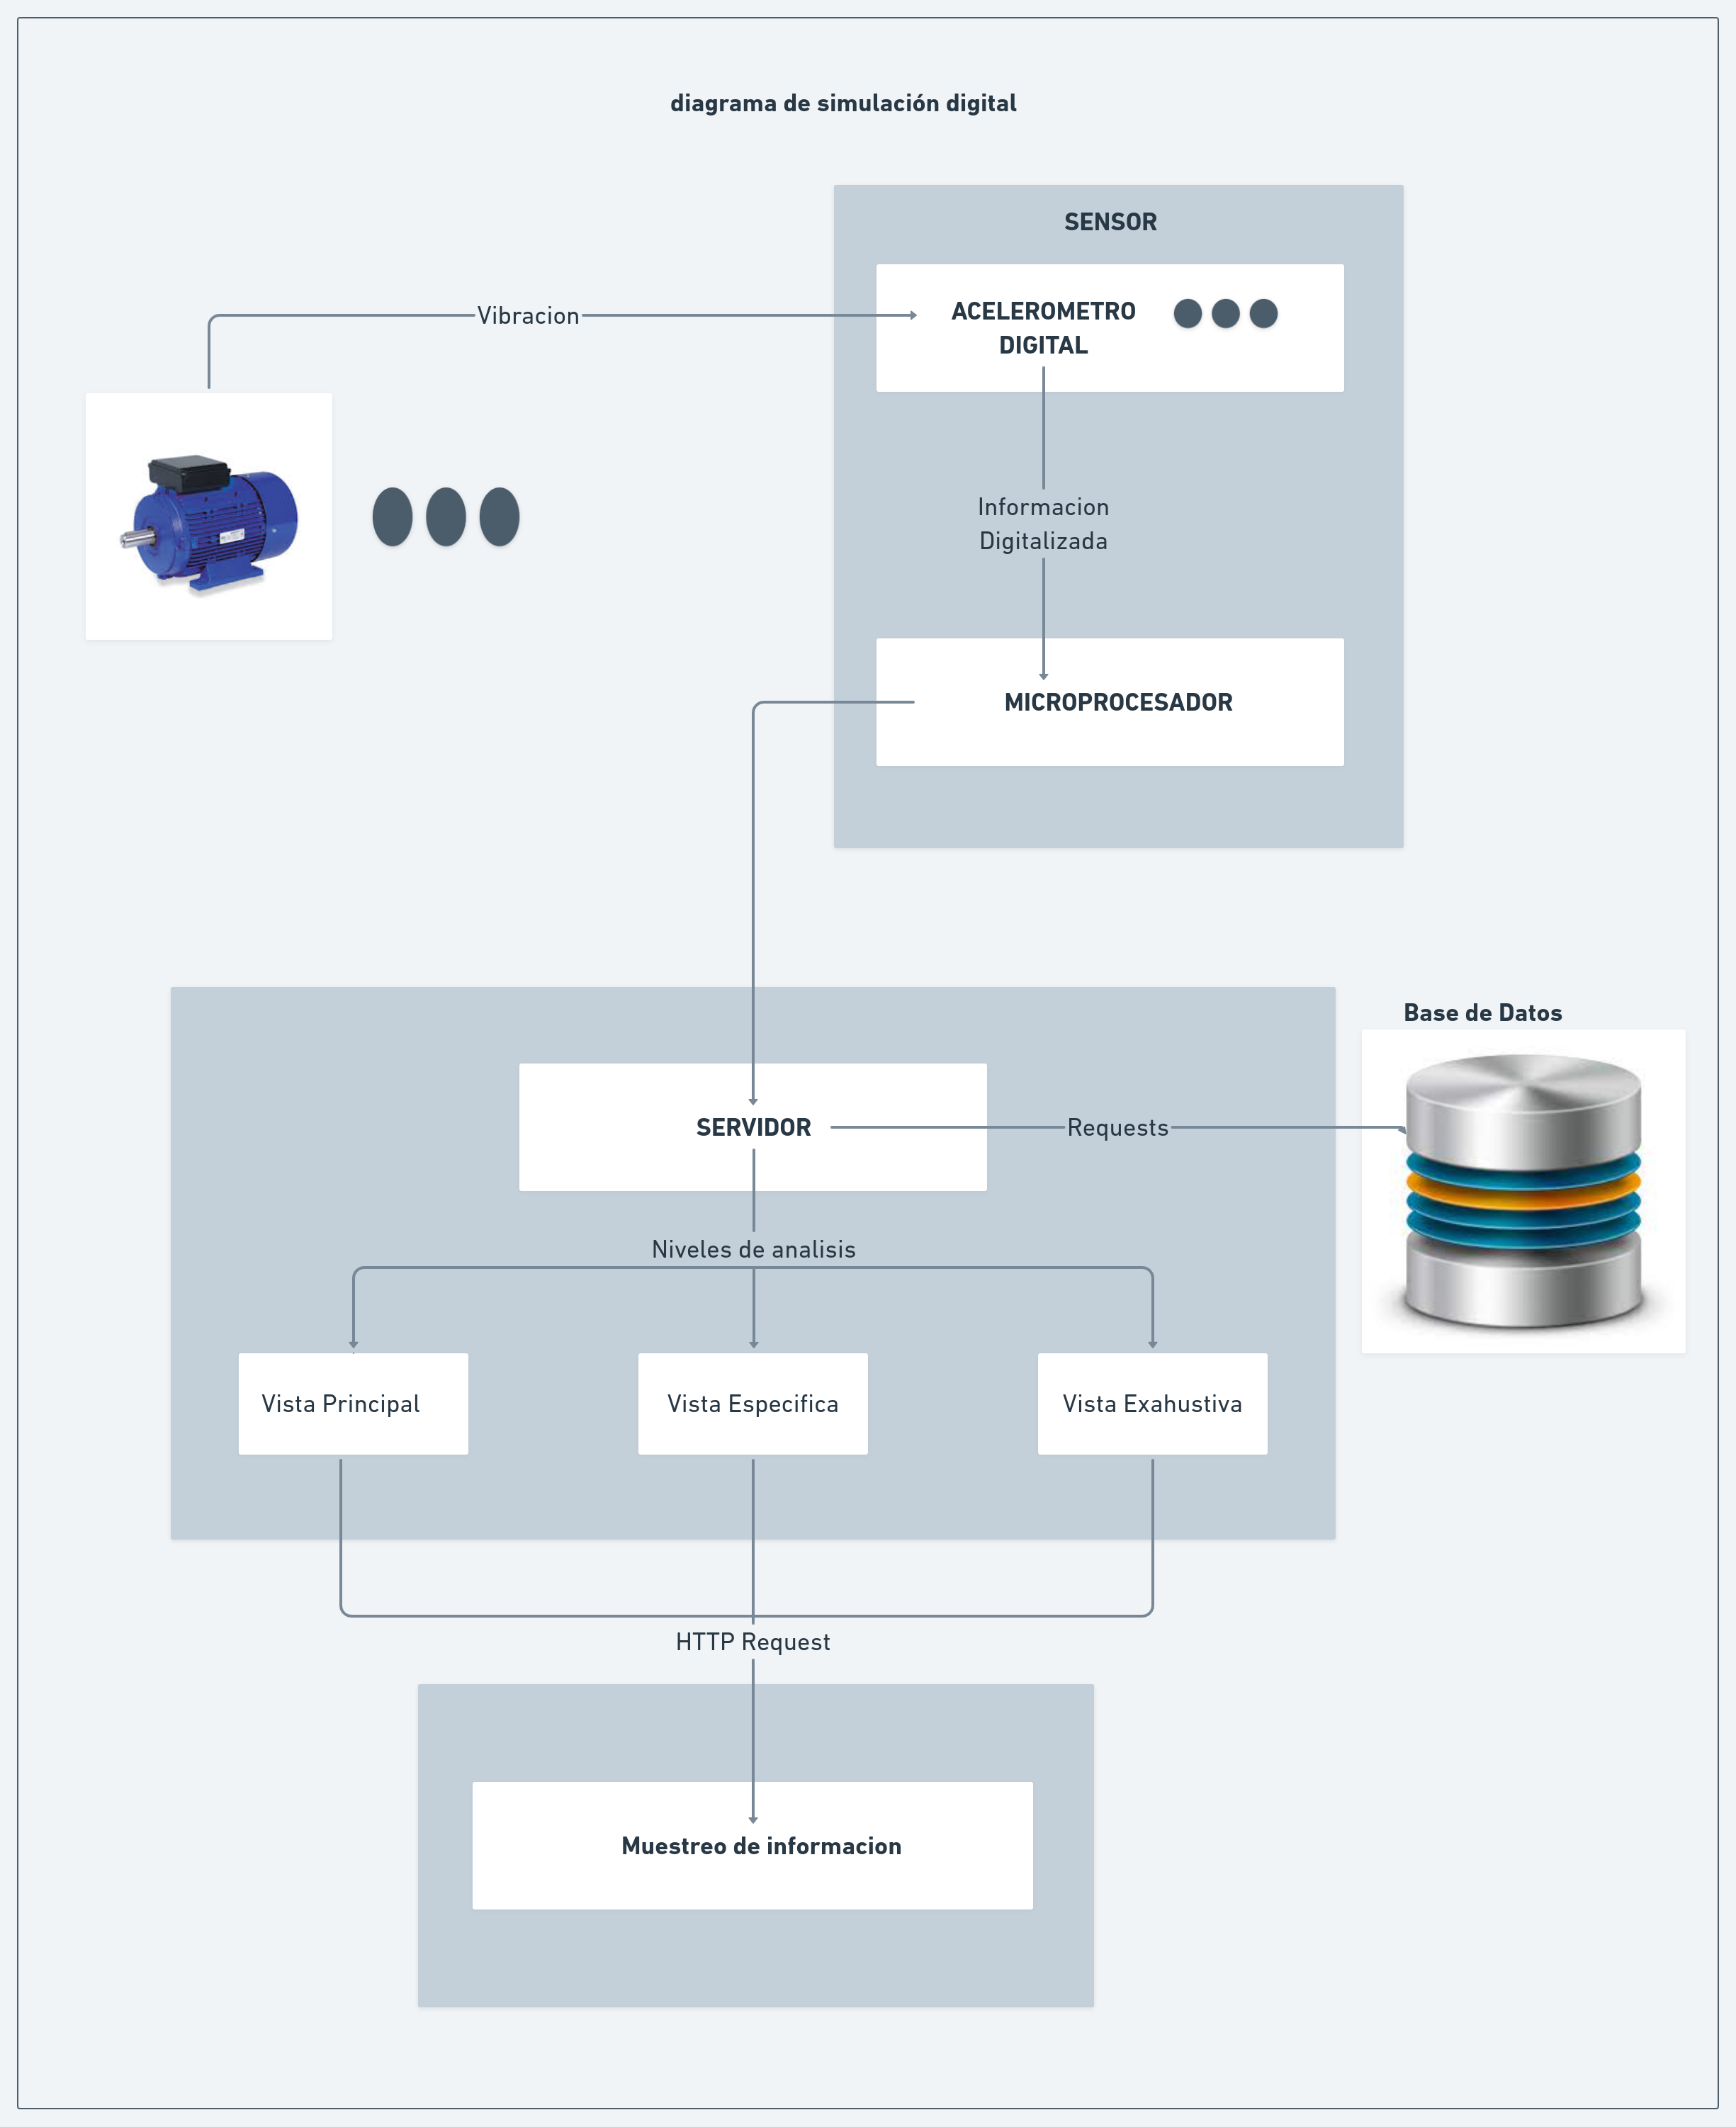
\includegraphics[width=15cm, height=23cm]{Diagrama_sensorica.png}
\end{figure}
